% This is samplepaper.tex, a sample chapter demonstrating the
% LLNCS macro package for Springer Computer Science proceedings;
% Version 2.20 of 2017/10/04
%
\documentclass[runningheads]{llncs}
%
\usepackage{graphicx}
\usepackage{booktabs}
\usepackage{cite}
\usepackage{url}
\usepackage{multirow}
\usepackage{pgfplots}
\usepackage{tikz}
\usetikzlibrary{matrix,fit,shapes,calc,positioning,shadows,arrows,shapes,backgrounds,decorations.markings,fadings}
\usepackage{listings}
\usepackage[caption=false, font=footnotesize]{subfig}
%%%%%%%%%%%%% code listing
\renewcommand{\ttdefault}{pcr}
\lstset{
  basicstyle=\scriptsize\ttfamily,
  keywordstyle=\scriptsize\ttfamily\bfseries,
  language=C,             % choose the language of the code
  frame=single,              % adds a frame around the code
  aboveskip=0pt,
  belowskip=0pt,
  breaklines=true,           % sets automatic line breaking
  breakatwhitespace=false,   % sets if automatic breaks should only happen at
  showspaces=false,
  %numbersep=5pt,              % Abstand der Nummern zum Text
  %tabsize=2,                  % Groesse von Tabs
  %extendedchars=true,         %
  %breaklines=true,            % Zeilen werden Umgebrochen
  keywords=[2]{tcp, flag, threshold, track, count, seconds, classtype, sid}
}
\usepackage{balance}
\usepackage{wrapfig}
\usepackage{enumitem}
\usepackage{color, colortbl}
\definecolor{Gray}{gray}{0.9}

\newcommand{\tname}{\textsc{Syrius}} %% name of the technique
\newcommand{\ie}{i.e.}
\newcommand{\eg}{e.g.}
\newcommand{\aka}{a.k.a.}
\newcommand{\etal}{and colleagues}
\newcommand{\nids}{NIDS}
\newcommand{\metas}{Metasploit}
\newcommand{\suri}{Suricata}
\newcommand{\numrulessuri}{27.8K}
\newcommand{\percRulesWithContent}{93.5\%}
\newcommand{\numundetected}{\Fix{XX\%}}
\newcommand{\CodeIn}[1]{{\small{\texttt{#1}}}}
\newcommand{\MyComment}[1]{}

%% review
\newcommand{\Fix}[1]{{\textbf{[[}\color{magenta}#1}\textbf{]]}}
\newcommand{\Mar}[1]{{\textbf{[[Marcelo:~}\color{red}#1}\textbf{]]}}
\newcommand{\Luc}[1]{{\textbf{[[Lucas:~}\color{blue}#1}\textbf{]]}}
\newcommand{\Gui}[1]{{\textbf{[[Guilherme:~}\color{green}#1}\textbf{]]}}

\def\denseitems{
   \itemsep1pt plus1pt minus1pt
   \parsep0pt plus0pt
   \parskip0pt\topsep0pt}

%% numbers
\newcommand{\totoptions}{162}
\newcommand{\numproto}{11}
\newcommand{\totoptionsrelevant}{153}


% Used for displaying a sample figure. If possible, figure files should
% be included in EPS format.
%
% If you use the hyperref package, please uncomment the following line
% to display URLs in blue roman font according to Springer's eBook style:
% \renewcommand\UrlFont{\color{blue}\rmfamily}

\begin{document}
%
\title{Synthesis of Rules for Network Intrusion Detectors}
%
%\titlerunning{Abbreviated paper title}
% If the paper title is too long for the running head, you can set
% an abbreviated paper title here
%
\author{Lucas Alcantara\Comment{\inst{1}}\Comment{\orcidID{0000-1111-2222-3333}} \and
Guilherme Padilha\Comment{\inst{1}}\Comment{\orcidID{1111-2222-3333-4444}} \and
Marcelo d'Amorim\Comment{\orcidID{0000-0002-1323-8769}}}
%
\authorrunning{Alcantara et al.}
% First names are abbreviated in the running head.
% If there are more than two authors, 'et al.' is used.
%
\institute{Federal University of Pernambuco (UFPE), Recife, Brazil\\
\email{\{lama,ghps,damorim\}@cin.ufpe.br}}
%
\maketitle              % typeset the header of the contribution
%
\begin{abstract}
Network Intrusion Detection Systems (\nids{}) are a popular mechanism
used by system administrators to defend against network attacks. These
systems monitor the network traffic and flag suspicious network
behavior. Signature-based \nids\ do that by checking the network
traffic against a pre-defined set of rules, which can become obsolete
as attackers learn new strategies to circumvent existing defenses.
This paper proposes \tname{}, a technique that automatically
synthesizes \nids\ rules from positive and negative examples (\ie{},
malicious and benign traffic). \tname{} formulates synthesis as an
optimization problem whose candidate solutions are rules that
maximizes the captured the positive traffic and minimizes the captured
negative traffic. \tname{} bootstraps the search with candidate
solutions that use data from the payload of the malicious message and
produces optimal rule candidates on output. We evaluated \tname{} on a
diverse set of attacks. Results indicate that \Fix{...}

%% optimizes the
%% candidate solution to capture the positive example and, and then
%% optimizes the candidate solution to avoid capturing the negative
%% traffic. 


\keywords{NIDS, synthesis, search}
\end{abstract}
%
%
%
\section{Introduction}

Network Intrusion Detection Systems (\nids{}) are software systems
that monitor the network traffic for malicious behavior and act
accordingly by blocking messages or alerting humans about suspicious
events~\cite{Mitchell:2014:SID:2597757.2542049}. \nids{} are typically
placed behind a firewall, vetting the traffic that the firewall did
not block. Various open-source (\eg{}, Snort~\cite{snort} and
Suricata~\cite{suricata}) and commercial NIDS implementations (\eg{},
SolarWinds~\cite{solarwinds} and IBM QRadar~\cite{qradar}) exist
today. These systems are very popular in industry to secure local
computer networks given the amount of potential malicious traffic that
exist on the Internet.

\sloppy \nids{} are typically categorized in two
groups~\cite{kumar2007survey}: rule-based and anomaly-based \nids. A
rule-based intrusion detector\footnote{\aka\ signature-based intrusion
  detector.} checks if the network traffic matches a fixed set of
rules. Figure~\ref{fig:synflood-example} shows an example rule of
Suricata~\cite{suricata}, a popular open-source \nids{}. This rule
prescribes a method to capture a denial-of-service
attack~\cite{understanding-dos} to a server by matching specific
conditions about the network traffic. Relevant properties about the
traffic of interest appear in bold (see
Section~\ref{sec:suri-metas-coverage}). Rule-based \nids{} focus on
known attacks whereas anomaly-based \nids{} focus on unknown attacks
that could be observed by first learning the regular traffic and then
acting
properly~\cite{kumar2007survey,Mitchell:2014:SID:2597757.2542049,cordy-etal-issta19}. These
two kinds of intrusion detection mechanisms are
complementary. Rule-based NIDS could miss attacks (as rulesets can
become outdated) whereas anomaly-based NIDS can raise false alarms (as
detection algorithms are approximate).

Rule-based NIDS are restricted to a fixed set of rules defined by the
network system administrator. Manually writing these rules is tedious,
error-prone, but important as attackers constantly create new
strategies to circumvent existing rules. IT-security companies
capitalize on this phenomena and put rulesets on the market for
sale~\cite{proofpoint-etpro,snort-rule-subscriptions}.  Despite this
fundamental issue, rule-based systems are tremendously popular in
industry today. Anomaly-based NIDS are not restricted to a fixed set
of rules. They learn usage behavior from positive traffic and, based
on that, alert uncommon behavior~\cite{7579764}. Unfortunately,
anomaly-based NIDS are fundamentally imprecise. To sum up, rule-based
NIDS are precise but incomplete whereas anomaly-based NIDS are (more)
complete but imprecise.

%% This paper focuses on the
%% problem of discovering new rules by using anomaly-based NIDS.

This paper proposes \tname{}, a technique that uses machine
intelligence to automatically synthesize rules for rule-based
\nids. Our general goal is to harden the protection of NIDS by
improving the creation process of rules. One scenario of application
of \tname{} is one where an anomaly-based NIDS identifies abnormal
traffic and signals that traffic to \tname{} to create and distribute
the rules.

%% Note that anomaly-based NIDS are evolving pretty quick with the
%% advances in machine learning, but rule-based NIDS are still extremely
%% popular.  \tname{} could also leverage existing databases of malicious
%% traffic to synthesize rules.  Regardless of how the negative traffic
%% is produced (out of scope of this paper), those rules can be
%% distributed to rule databases for free.
%%  The
%% core motivation is that 1) attackers are productive in creating new
%% ways to circumvent existing protections and 2) manual creation of
%% rules is tedious and time-consuming.  

\tname{} synthesizes rules from positive and negative examples, \ie{},
malicious and benign traffic.

\Fix{summarize how the technique works}

\Fix{summarize results}

This paper makes the following contributions.

\section{Background}

This paper focuses on signature-based \nids, Suricata, in
particular. But the principles we use are general to any other
signature-based \nids~(\eg{}, Snort~\cite{snort}).

\subsection{Suricata Rules}
\label{sec:example-suricata-rules}

Figure~\ref{fig:synflood-example} shows an example rule of
Suricata~\cite{suricata}, a popular open-source \nids{} maintained by
the Open Information Security Foundation (OISF)~\cite{oisf}. A
Suricata rule is divided in three parts---action, header, and rule
options~\cite{suri-rule-format}. The action part appears as the first
word in the rule description. An action denotes the task that needs to
be executed if the rule pattern is satisfied. In this example, a
message will be sent to system administrators if the rule pattern is
satisfied. The header comes after the action in the rule
description. It restricts the information flow covered by the
rule. For this rule, the header is \CodeIn{tcp \$HOME\_NET any ->
  \$EXTERNAL\_NET any}. It instructs Suricata to inspect \CodeIn{tcp}
traffic flowing from any port in the home network to any other address
outside the home network. The variables \CodeIn{\$HOME\_NET} and
\CodeIn{\$EXTERNAL\_NET} are configurable. The rule options come after
the header. It is a semi-colon-separated sequence of key-value
pairs. Some options serve to document the analyzed traffic (\eg{},
``msg'', ``classtype'', and ``sid'') whereas the remaining properties
describe characteristics of the attack (\eg, ``flags'', ``threshold'',
and ``content''). The main challenge in synthesizing rules is to
discover the set of options that make a rule to capture the malicious
traffic, but ignore the benign traffic.

\begin{table}[h]
  \caption{\label{table:rules}Supported options}  
  \centering
  \begin{tabular}{lllll}
    \toprule
    \multicolumn{1}{c}{\#} & \multicolumn{1}{c}{Option} &  \multicolumn{1}{c}{Description}\\
    \midrule     
    1 & dsize & matches on the size of the packet payload\\
    2 & itype & matches on a specific ICMP type\\
    3 & icode & matches on a specific ICMP code\\
    4 & icmp\_seq & checks a ICMP sequence number\\
    5 & icmp\_id & matches on specific ICMP id-values\\
    6 & window & check for a specific TCP window size\\
    7 & flags & matches on TCP flags\\
    8 & fragbits & checks if the fragmentation or reserved bits are set in the IP header\\
    9 & threshold & used to control the rule’s alert frequency\\
    10 & content & matches on bytes of the payload\\
    \bottomrule
  \end{tabular}
\end{table}


\section{Illustrative Examples}
\label{sec:suri-metas-coverage}

\begin{figure}[t]
  \lstinputlisting[language=C,numbers=none,keywords={flags,threshold}]{synflood.suricata}
  \caption{Suricata rule for SYN Flood Attacks.}
  \label{fig:synflood-example}
\end{figure}

This section briefly presents examples of attacks and rules that are
synthesized with \tname{} to capture those attacks.

\subsection{SYN Flood Attack}

The SYN Flood attack exploits a vulnerability in the TCP/IP handshake
to establish a TCP connection~\cite{cloudfare-synflood}. The handshake
works as follows in normal circumstances. First, a client sends a SYN
packet to the server, requesting a connection. Second, the server
responds with a SYN-ACK packet to the client. Third, the client
responds with an ACK message and the connection is established. Aware
of the protocol, an attacker sends multiple SYN packets to different
ports of a server, often using fake IP addresses. Then, after the
server responds with a SYN-ACK packet, the client keeps sending other
SYN packets to avoid the connection to time out. Without proper
protection, the server accepts these malicious requests and eventually
legitimate requests cannot be satisfied due to resource exhaustion.
Figure~\ref{fig:synflood-example} shows a Suricata rule to capture
this attack. The critical parts appear in bold---the option
\CodeIn{flags: S,12}, which identifies a SYN packet and the option
\CodeIn{threshold: type both, track by\_dst, count 5000, seconds 5},
indicating that a high volume of such packets should be requested in a
short period of time.

%\Mar{please, explain the other fields}

\subsubsection{\tname\ on SYN Flood Attack}

\Mar{Guilherme/Lucas (CRI): we need to show how \tname{} works on this
  example. What is the input? How long does it take to generate the
  rule? Is the rule generated exactly the same? Please explain...}


\Fix{repeat this for two other attacks. one non-dos/flood non-content}
  

\section{Technique}

\tname{} is a technique that uses positive and negative examples to
synthesize signature-based NIDS rules, such as those from Snort and
Suricata. The goal of \tname\ is to create a rule that \emph{only}
captures the positive traffic, \ie{}, the malicious sequence of
messages. 

\vspace{1ex}
\noindent\textbf{Overview.}~\tname{} synthesizes rules in two
steps. First, it produces a potentially overspecified rule that
captures the malicious traffic provided on input. In this step,
\tname\ \emph{maximizes} the number of options in the rule that
captures the positive traffic. It extracts tokens from the malicious
message and use them to define the initial rule. Furthermore, it
searches for additional rule option (\eg, \Fix{xxx}) that are not
found in the message data but are satisfied by the traffic. We say
that this rule overfits the problem as it clearly satisfy the success
criterion of only capturing the positive traffic, however it is unable
to generalize to other attacks of the same kind with different
data. In the second step, \tname{} uses negative examples to
\emph{minimize} the rule, discarding unnecessary options. Note that
any subset of options in the rule obtained in this stage captures the
positive traffic by construction. \Fix{...elaborate...}

\subsection{Step 1: Rule Maximization}
\pgfplotsset{width=6cm,compat=1.8}
\pgfplotsset{every tick label/.append style={font=\tiny}}

The goal of the first step is to synthesize a rule with the maximum
number of options that satisfy the malicious traffic. A rule is
maximal if no other option can be added without missing the malicious
traffic.

\begin{wrapfigure}[16]{r}{0.5\textwidth}
  \centering
  \vspace{-5ex}
  \scalebox{1.05}{
    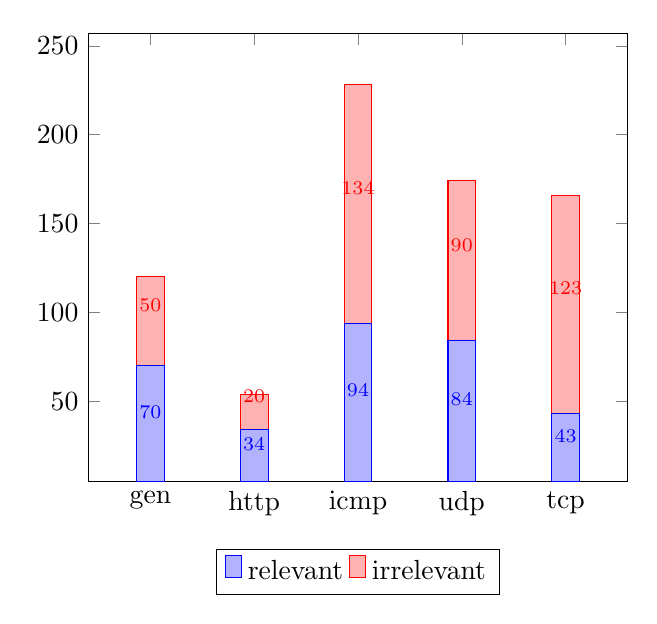
\begin{tikzpicture}
      \begin{axis}[
          ybar stacked,
          enlargelimits=0.15,
          legend style={at={(0.5,-0.15)},
            anchor=north,legend columns=-1},
%          ylabel={\#rules},
          symbolic x coords={gen, http, icmp, udp, tcp},
          xtick=data,
          nodes near coords,
          every node near coord/.append style={font=\scriptsize},        
          nodes near coords align={vertical},
        ]
        \addplot coordinates {(gen,70) (http,34) (icmp,94) (udp,84) (tcp,43)};
        \addplot coordinates {(gen,50) (http,20) (icmp,134) (udp,90) (tcp,123)};    
        \legend{relevant, irrelevant}
      \end{axis}
    \end{tikzpicture}
  }
  \caption{\label{fig:distribution-rules-protocol}Distribution of
    number of rules per protocol and relevance for triggering action.}
\end{wrapfigure}
It is important to note that options can be specific to a given
protocol or general and they can influence or not triggering an
action. The purpose of rule options \CodeIn{msg}, for instance, is to
print on the output an informative message indicating what kind of
intrusion has been
observed. Figure~\ref{fig:distribution-rules-protocol} shows the
distributions of these options per protocol and their relevance for
triggering rule actions. We obtained this information
by\Fix{...explicar como...} \Fix{eh um pouco suspeito ter tantas regras
  irrelevantes...}This plot indicates that the problem search
space is defined based on the protocol of the malicious traffic. For
instance, if \tname{} detects by analyzing the format of network packets that the attack involves \CodeIn{http}
traffic, then 34 different rule options will be considered in the
creation of the rule.

To infer options, \tname{} parses the protocol message, looking for
fields in the message associated with options. For example, fields
\Fix{...and...}  can be used to determine the option
\Fix{...}. Unfortunately, inferring options at the field granularity
level is insufficient to capture \CodeIn{content} options (see
Section~\ref{sec:example-suricata-rules}), which refer to parts of the
payload of the message and cannot be directly extracted directly from
the fields. Handling this case is critically important as most rules
contain \CodeIn{content} options. Figure~\ref{fig:distribution-contents} shows
the histogram of number of these options per rule (up to 10) for the
Suricata public rule database \Fix{cite}. Rules without \CodeIn{content}
options is an exception and half of the rules contain at least two
\CodeIn{content} options.
\begin{wrapfigure}[14]{r}{0.56\textwidth}
  \centering
  \vspace{-3ex}
  \scalebox{1.2}{  
    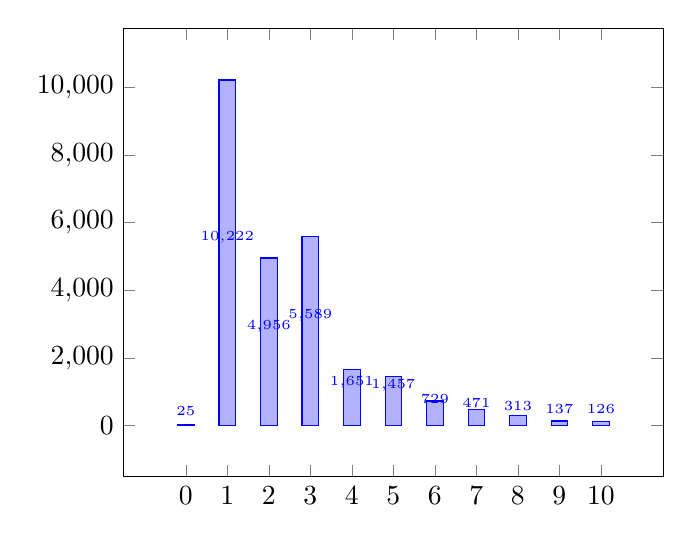
\begin{tikzpicture}
      \begin{axis}[
          bar width=6pt,
          scaled ticks=false,
          tick label style={/pgf/number format/fixed},
          ybar stacked,
          enlargelimits=0.15,
          legend style={at={(0.5,-0.15)},
            anchor=north,legend columns=-1},
          symbolic x coords={0, 1, 2, 3, 4, 5, 6, 7, 8, 9, 10},
          xtick=data,
          nodes near coords,
          every node near coord/.append style={font=\tiny},
          nodes near coords align={vertical},
        ]
        \addplot coordinates {(0,25) (1,10222) (2,4956) (3,5589)
          (4,1651) (5,1457) (6, 729) (7, 471) (8, 313) (9, 137) (10, 126)};
      \end{axis}
    \end{tikzpicture}
  }
  \caption{\label{fig:distribution-contents}Histogram of number of
    \CodeIn{content} options per rule (up to 10).}
\end{wrapfigure}
To find the values associated with these options, \tname{} splits the
payload of the malicious message in tokens using natural language
delimiters, such as $\backslash$t, $\backslash$n, $\backslash$r, and
spaces. The rationale for this decision is that we observed, by
inspecting existing rules, that \CodeIn{content} options typically refer to
sequence of characters in the payload of messages separated by these
delimiters. \Fix{describe extraction of options not in the
  message. give examples! search only makes sense if this exists!}

\subsection{Step 2: Rule Minimization}

The rule reported by the first step satisfies the criterion to only
capture positive traffic, however it is ``too'' specific---it is
unable to capture different manifestations of the same attack as the
rule would unlikely match exactly the options we found for the input
message. Some options added to the rule during the first step are
irrelevant for determining the attack and should be removed.

The goal of this step is to create a \emph{minimal} rule that captures
\emph{only} the positive malicious traffic. A rule is minimal if
discarding any option results in capturing negative (\ie{}, benign)
traffic. Recall that the previous maximization step produces a rule
that captures the positive traffic and all options are satisifed by
the positive traffic. Consequently, any subset of these options also
captures the positive traffic. The minimization procedure we propose
in this step builds on that observation. It iteratively discards
options from the candidate rule until no other options can be
removed. The procedure uses negative traffic to guide the
search. Public databases of negative traffic with \Fix{thousands} of
messages exist \Fix{cite cite} and can be used to increase the
accuracy of the minimization.


\Fix{...............estou aqui}

%% \begin{figure*}[t]
%% \centering
%% 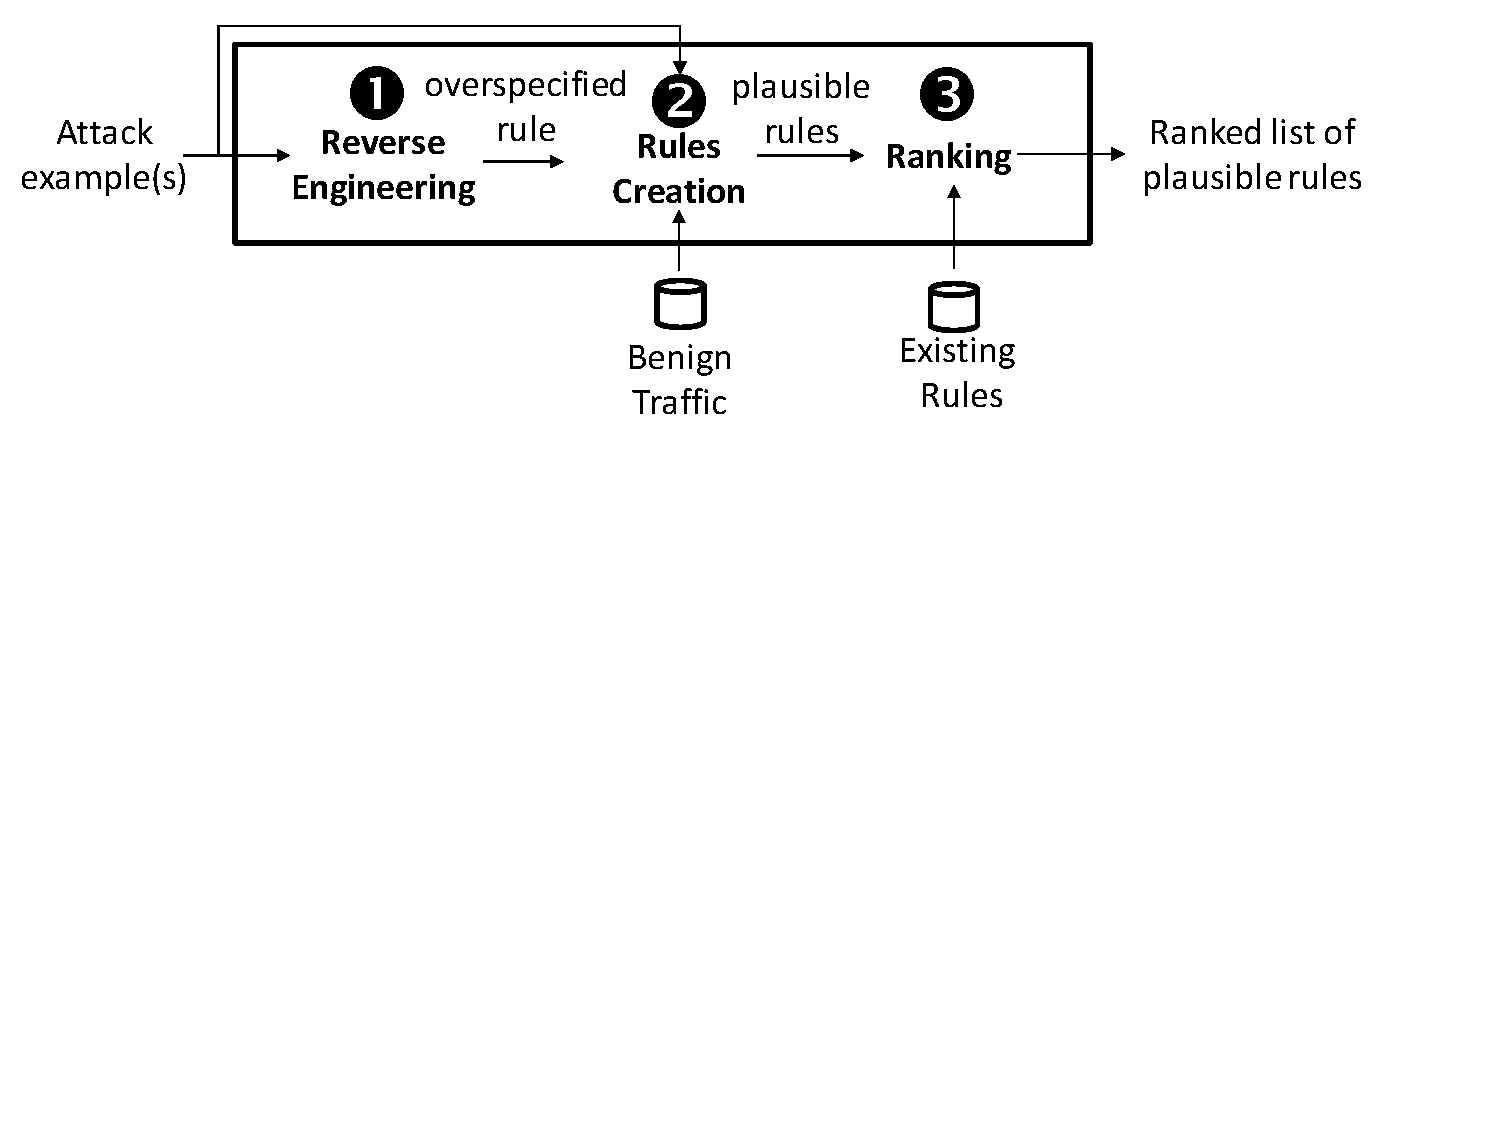
\includegraphics[trim=10 360 182 130,clip,width=0.95\textwidth]{figs/nids-workflow}
%% \caption{\tname\ workflow.}
%% \label{fig:overview}
%% \end{figure*}

Figure~\ref{fig:overview} shows the workflow of \tname{} as a pipeline
of two components, appearing numbered in the figure. Each component
implements one of the steps mentioned above. The goal of the first
component is to produce a rule that captures the negative traffic.
First, it initializes the rule with random values. Only options
associated with the used protocol are included in the rule
representation. Then, \tname\ optimizes the rule options until
\suri\ is able to capture the attack associated with the negative
traffic.  \tname\ unsuccessfully terminates at this point if it cannot
capture the attack. The second component takes as input the rule
produced by the first component and tries to minimize that rule. Note
that any subset of options would capture the negative traffic---as all
options in the rule need to be satisfied for the negative traffic to
be captured---but it can also capture positive traffic. This component
systematically discards options from the rule encoding until no
positive traffic is captured.

\subsection{Problem Characterization}

One important step in search-based optimization is to characterize a
candidate solution to the target problem. Candidate solutions are the
objects that the search optimize towards solutions. In this case, a 
candidate solution is an encoding of a Suricata rule.  \tname\ encodes
the rule options segment of a Suricata rule (see
Section~\ref{sec:example-suricata-rules}) as a vector of Option
objects. Some options are discarded as they only serve for
documentation. For example, the options \CodeIn{msg},
\CodeIn{classtype}, and \CodeIn{misc-activity}, appearing in the
example on Figure~\ref{fig:synflood-example}, have no influence in
triggering the actions associated with the rule. The option
\CodeIn{flags}, however, is relevant to trigger the action. \tname{}
models that option with a data structure storing two fields, one of
character type and another of integer type. This enables \tname{} to
mutate each element separately. Similar encodings are used in modeling
the other relevant options. We found what options are (ir)relevant by
inspecting Suricata code for the presence of \CodeIn{eval} functions,
which are invoked from a main loop to process each action rule. The
presence of such a function for a given option indicates that it is
relevant for triggering some action of some rule.

\subsection{Initial State}

To bootstrap the search, \tname{} needs to select an initial
solution. When creating such candidate solution, \tname{} first looks
for the protocol related to the malicious input traffic. Then, it
selects the relevant options for that protocol and initializes the
option vector with default values. \Mar{Suricata define valores
  default?  Vcs. definiram?  Isto foi baseado em popularidade ou o
  que?}

%% \tname{}
%% uses an abstract representation of a Suricata rule that reflects the
%% concrete representation of the rule. The concrete rule representation
%% is the one actually used by Suricata whereas the abstract
%% representation is the one \tname{} uses to run the search.

\subsection{Fitness Functions}

The fitness value of a candidate solution $c$, modeling the rule
options $o_1, \dots, o_n$ is given by $f(c)=1-\Sigma{d(o_i,m)}/n$,
where $i$ ranges from 1 to $n$ and $m$ denotes the negative
traffic. The higher the fitness value the better, \ie{}, the fitter
the candidate solution $c$ will be.  The value of the expression
$d(o_i,m)$, associated with option $o_i$, ranges over
0-1. Consequently, the value of the expression $\Sigma{d(o_i,m)}/n$
itself is in the 0-1 range, as there are $n$ options, and the range of
the function is 0-1.

As usual, we used customized distance functions to compute $d(o_i,
m)$. For example, let us consider the \CodeIn{flags} option, discussed
on Figure~\ref{fig:synflood-example}. Recall that this option
identifies the SYN packet in the tcp protocol and that its encoding in
\tname{} stores two attributes---one categorical and one
numerical. The value of $d(o_i, m)$, in this case, is obtained by
computing the normalized Euclidean distance in the two-dimensional
space. Considering that each of the two dimensions has cardinality of
ten, the distance of a candidate solution holding the option
\CodeIn{flags(S,13)} to the solution will be 0.22
(=$1/\sqrt{20}$). Note that the smaller the distance the better.

\tname{} uses a modified version of Suricata to measure distance. It
updates the rule set that the modified version of Suricata analyses,
injects the traffic on the network, and monitors the execution. Each
rule option has an associated \CodeIn{eval} function in code. \tname{}
monitors the execution of these functions to identify how far it is
from returning true, which indicates it is closer to trigger the
action associated with the rule. 
\Luc{Originalmente, o suricata interrompe a checagem de uma regra quando alguma das opções não dá match com o pacote analisado. O código fonte foi alterado para que as regras sempre tenham todas as suas opções verificadas. A função de verificação de uma opção retorna um booleano indicando se o valor da opção na regra corresponde ou não ao valor da opção no pacote. Para opções cujos valores são numéricos, alteramos o código fonte para obter a diferença entre os valores da opção na regra e no pacote.
\\*
Exemplo trecho de código original opção "icode":

\begin{figure}[h]
  \lstinputlisting[language=C,numbers=none,keywords={}]{original.code}
  \caption{Original source code.}
  \label{fig:original-code}
\end{figure}

Trecho modificado:

\begin{figure}[h]
  \lstinputlisting[language=C,numbers=none,keywords={}]{modified.code}
  \caption{Modified source code.}
  \label{fig:modified-code}
\end{figure}
    
}

\Fix{Lucas/Guilherme, it would be good to show how this looks like in
  code}

\subsection{Search}

\tname{} is a single-individual hill-climbing like search.


\subsection{Limitations}

\Fix{...}

\section{Evaluation}

%% \renewcommand{\labelitemi}{}
%% \setitemize[0]{leftmargin=20pt,itemindent=-20pt}
%% \begin{itemize}
%% \end{itemize}

%% \renewcommand{\labelitemi}{}
%% \setitemize[0]{leftmargin=0pt,itemindent=0pt}
%% \begin{itemize}
%%   \item{\textbf{RQ1.}~How precise is \tname?}
%%   \item{\textbf{RQ2.}~How efficient is \tname?}
%% \end{itemize}

This section reports precision and efficiency of \tname.


\subsection{Objects of Analysis}

We evaluated \tname{} on a set of attacks covering each of the four
protocols supported by Suricata and attacks with different
characteristics. Table~\ref{table:attacks} shows the attacks we
analyzed and the rule of Suricata that captures the attack. Column
``Name'' shows the name of the attack, column ``\#'' indicates whether
single or multiple messages are required to manifest the attack,
column ``Protocol'' shows the protocol name, column ``Description''
summarizes the effect of the attack, if successfull, and column
``Golden Rule'' shows the relevant parts in the options section of the
Suricata rule that captures the attack.

\begin{table*}[t!]
  \caption{\label{table:attacks}Characterization of attacks analyzed
    and Golden Rule of Suricata (reference) to capture it.\Mar{please,
  show me the Golden Rule, \ie{} the part that is relevant of each rule (for
  capturing the negative traffic precisely)}}  
  \centering
  \begin{tabular}{lllll}
    \toprule
    \multicolumn{1}{c}{Name} & \multicolumn{1}{c}{\#} & \multicolumn{1}{c}{Protocol} & \multicolumn{1}{c}{Description} & \multicolumn{1}{c}{Golden Rule} \\
    \midrule     
    Ping Scan & single & ICMP & Discovers active hosts in a network &  dsize:0; itype:8; \\
    Black Nurse & multiple & ICMP & Denial of Service & itype:3; icode:3; detection\_filter:track by\_dst, count 250, seconds 1;\\
    Ping Flood  & multiple & ICMP & Denial of Service & itype:8; icode:0; detection\_filter:track by\_src, count 30, seconds 1;\\  
    Port Scan TCP & single & TCP & Discovers open ports in a host & flags: A; ack: 0;dsize: 0; \\
    SYN Flood & multiple & TCP & Denial of Service & flags: S,12; threshold: type both, track by\_dst, count 5000, seconds 5;\\
    UDP Flood & multiple & UDP & Denial of Service & fragbits:M; threshold: type both, track by\_dst, count 5000, seconds 5; \\
    \bottomrule
  \end{tabular}
\end{table*}

\subsection{Setup}

Note from Figure~\ref{fig:overview} that the negative traffic is an
input to the technique. The positive (non malicious) traffic, in
contrast, is not. \tname{} uses public databases storing different
kinds of positive traffic for all protocols covered by Suricata. We
used two datasets of positive traffic. The Bigflows.pcap dataset is
part of the TcpReplay~\cite{tcpreplay} open source project. This
dataset includes real network traffic on a busy private network access
point to the Internet. According to the TcpReplay web site ``This
capture is much larger and has a smaller average packet size than the
previous capture (smallFlows.pcap). It also has many more flows and
different applications.''. In addition to the Bigflows.pcap dataset,
we also used datasets of normal traffic made available by Stratosphere
Lab~\cite{stratosphere-normal}.

%% \Gui{We are using the bigflows.pcap provided by tcpreplay on http://tcpreplay.appneta.com/wiki/captures.html "This is a capture of real network traffic on a busy private network’s access point to the Internet"
%%  }

\Luc{entrada: utilizamos a ferramenta hping3 para executar o ataque em um alvo arbitrario dentro da rede (n ha necessidade de haver um alvo real para executar o hping3) e capturamos o trafego gerado com o wireshark. o comando utilizado foi:\\*
\texttt{\# hping3 -d 80 -w 64 -S -p 80 --flood --rand-source 192.138.1.115} \\*
que envia pacotes de 80 bytes (-d 80), com a flag SYN habilitada (-S), tamanho de janela de 64 bytes (-w 64), direcionados a porta 80 (-p 80). A flag --flood indica q o hping3 vai enviar os pacotes o mais rápido possível. a flag --rand-source indica que cada pacote vai ter um ip de origem aleatorio. 192.138.1.115 é o alvo.\\*
O trafego armazenado contem 40 mil pacotes SYN, enviados no intervalo de 1 segundo,  pegamos uma amostra de 20 desses pacotes para representar o flood e servir como entrada.\\*
O wireshark armazena os pacotes no formato pcap, utilizamos a ferramenta tcpreplay para reproduzir o trafego com o comando:\\*
\texttt{\# tcpreplay --pps 200 --intf1=wlp2s0 Datasets/syn-flood-sample.pcap}\\*
Nesse caso, estamos enviando os pacotes armazenados em \texttt{Datasets/syn-flood-sample.pcap} a uma taxa de 200 pacotes por segundo (\texttt{-pps 200}) utilizando a interface wlp2s0 (\texttt{--intf1 wlp2s0})\\* 
Há diferenças entre os pacotes na opção ack.\\* 
Por que 20? Apenas para gerar a regra mais rapidamente, poderia ser qualquer valor maior ou menor. No final, o parâmetro \texttt{count} da opção \texttt{threshold} vai ser alterado pelo adm da rede.\\*
Intervalo de reprodução: 0.005 segundo


\begin{table}[h]
  \caption{\label{table:rules}Rule evolution}  
  \centering
  \begin{tabular}{lllll}
    \toprule
    \multicolumn{1}{c}{Iteration} & \multicolumn{1}{c}{Rule} \\
    \midrule     
    0 & (ack:0; seq:0; window:0; flags:F;)\\
    5 & (window:0; flags:F;)\\
    68 & (window:64; flags:F;)\\
    73 & (window:64; flags:S,12;)\\
    94 & (window:64; flags:S,12; threshold: type both, track by\_dst, count 20, seconds 1;)\\
    \bottomrule
  \end{tabular}
\end{table}

}

\Fix{any other detail we should consider?}

\subsection{Precision}

\Fix{...}

\subsection{Efficiency}

\Fix{...}

\section{Threats to Validity}

External Validity. \Fix{elaborate ...how popular are Suricata/Metasploit?}

\section{Related Work}

\Fix{...}
%
% ---- Bibliography ----
%
% BibTeX users should specify bibliography style 'splncs04'.
% References will then be sorted and formatted in the correct style.
%
\bibliographystyle{splncs04}
\bibliography{references}
%

\end{document}
